
\section{About}


%%%%%%%%%%%%%%%%%%%%%%%%%%%%%%%%%%%%%%%%%%%%%%%%%%%%%%%%%%%%%%%%%%%%%%%%%%%%%%%%%%%
%%%%%%%%%%%%%%%%%%%%%%%%%%%%%%%%%%%%%%%%%%%%%%%%%%%%%%%%%%%%%%%%%%%%%%%%%%%%%%%%%%%


\subsection{Hard Facts}

My name is Christoph Pickl and was born September 25th 1985 in
Burgenland/Austria. I usually have more than a few occupations at the same
time, so I am for example a student, musician, software developer, software
architect, tutor and from time to time a freelancer.
You can contact my any time for any reason via my mail address: e 0525580 -AT-
student.tuwien -DOT- ac.at


%%%%%%%%%%%%%%%%%%%%%%%%%%%%%%%%%%%%%%%%%%%%%%%%%%%%%%%%%%%%%%%%%%%%%%%%%%%%%%%%%%%
%%%%%%%%%%%%%%%%%%%%%%%%%%%%%%%%%%%%%%%%%%%%%%%%%%%%%%%%%%%%%%%%%%%%%%%%%%%%%%%%%%%


\subsection{Hobbies}

Following things I prefer to do in my sparetime besides any computer related
stuff:

%%%%%%%%%%%%%%%%%%%%%%%%%%%%%%%%%%%%%%%%%%%%%%%%%%%%%%%%%%%%%%%%%%%%

\subsubsection{Music}

\zitat{Also wer sagt dass er real ist und wer ist es echt.}

I am listening to a lot of different genres: Oldskool US HipHop (KRS-One, Jeru
the Damaja), German HipHop (Blumentopf, Beginner), Reggae (Anthony B,
Eek-a-Mouse), Dancehall (TOK, Red Rat), Reggaeton (Tony Touch), Jungle
(Aphrodite), Drumnbass (Renegade Hardware, JumpUp stuff), (Progressive) House,
Classic (Vivaldi, Bach), Electro (Daft Punk, Chemical Brothers), Easy Listening
(Yann Tiersen, Tracy Chapman), Aternative (Regina Spektor, Lilly Allen), Folk (Buena Vista Social Club),
\ldots~Depending on my mood I sometimes prefere the one or the other.

%%%%%%%%%%%%%%%%%%%%%%%%%%%%%%%%%%%%%%%%%%%%%%%%%%%%%%%%%%%%%%%%%%%%

\subsubsection{Turntablism}

\begin{figure}[htb]
    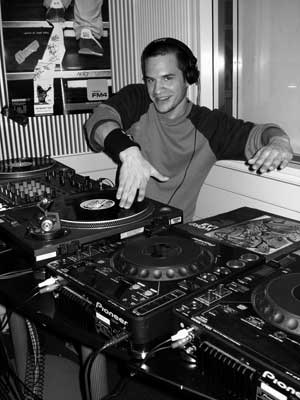
\includegraphics{img/Christoph_Pickl_at_FM4.jpg}
    \caption{Loves to spin the wheels of steel for the H{\"o}rspiel Crew}
\end{figure}

Since the early age of 16 he regularly practices his DJing and
turntablism skills. By the year of 2002 he joined the Austrian Rap crew
H{\"o}rspiel Crew\cite{hsc}. Since then, they released two albums and had gigs
at some famous festivals like Frequency or the Nuke festival.
%%%%%%%%%%%%%%%%%%%%%%%%%%%%%%%%%%%%%%%%%%%%%%%%%%%%%%%%%%%%%%%%%%%%

\subsubsection{Fitness}

\zitat{Nur in einem gesunden K{\"o}rper wohnt auch ein gesunder Geist.}

Sitting in front of the screen all day made me think of my health and therefore
decided to join a fitness club in Vienna. Since then I regularly (at least 3
times a week) visit Holmes Place in the 1$^{st}$ disrict.

%%%%%%%%%%%%%%%%%%%%%%%%%%%%%%%%%%%%%%%%%%%%%%%%%%%%%%%%%%%%%%%%%%%%

\subsubsection{Swimming}

Everyone, and especially my doctor, tells me just too often how important sport
is and so I have choosen to go swimming on a regularly base. The decision was
easy because water is such a great element (I like the sea a lot) and its a
safe and healthy sport too.

In the past, I did some other kinds of sport like skateboarding (as an extreme
sport, that one can be very painful) and basketball (although no extreme sport
can be nevertheless quite painful too) but somehow today there is not the time
for such things anymore \ldots


%%%%%%%%%%%%%%%%%%%%%%%%%%%%%%%%%%%%%%%%%%%%%%%%%%%%%%%%%%%%%%%%%%%%%%%%%%%%%%%%%%%
%%%%%%%%%%%%%%%%%%%%%%%%%%%%%%%%%%%%%%%%%%%%%%%%%%%%%%%%%%%%%%%%%%%%%%%%%%%%%%%%%%%


\subsection{Computer Interests}

\zitat{Das Ganze ist mehr als die Summe seiner Teile.}

Obiously, a computer science student have a lots of interest in technical
stuff; or at least, he should have :)

I personally do not like the hardware side -physics is really exciting,
yes, but for me it was never something I could fully understand- but prefer the
software and theoretical side of computers. Especially computer languages and
developing any kind of software, the theoretical background and simple but
powerfull user interfaces are things I am interested in.

A friend and I also founded the Java Student User Group \cite{jsug} in the year
2008 which serves as a platform from students for students which are heavily
interested in programming, Java and software development in general. As to
mention Java: That is something what is around me all day and everywhere these
days; University, work and private projects, which allows me to benefit
from the synergetic effect.

%%%%%%%%%%%%%%%%%%%%%%%%%%%%%%%%%%%%%%%%%%%%%%%%%%%%%%%%%%%%%%%%%%%%

\subsubsection{Languages}

\begin{itemize}
    \item Java, AspectJ, Scala
    \item C(++), C\#, Objective-C
    \item Smalltalk, Eiffel
    \item (J|P)ython, (J)Ruby, Groovy
    \item Perl, VB(A)
    \item ActionScript, AppleScript, shell scripting
    \item Haskell, Prolog
    \item SQL, PL/SQL
    \item XML\&Co, UML, LaTeX
    \item HTML, CSS, JavaScript
    \item JSF, JSP, PHP, ASP, CFML 
\end{itemize}

%%%%%%%%%%%%%%%%%%%%%%%%%%%%%%%%%%%%%%%%%%%%%%%%%%%%%%%%%%%%%%%%%%%%

\subsubsection{Topics}

\begin{itemize}
    \item Software Development
    \item Software Architectures
    \item Computer Languages
    \item OOP-AOP-FOP-LOP
    \item Free Open Source Software
    \item Filthy Rich User Experiences
    \item Software Configuration Management
    \item Dependency Injection
    \item Test Driven Development
    \item (strict) Coding Guidelines
    \item Code Quality Management
    \item Model Driven Software Development
    \item Design by Contract
    \item Relational Database Management Systems
    \item Object Oriented Databases
    \item Agile Software Development
    \item ... and generally new stuff I do not know yet.
\end{itemize}

\code{some_test.java}

%\lstinputlisting[<Optionen>]{pfad/zur/datei.php}
%\lstinline[<Optionen>]{hier kommt der Quellcode...}
